\chapter{Cotas comunes anidadas}

Retomamos el problema de admisión a universidades con cotas comunes igual que como se plantea en el capíitulo 7, se agrega la restricción de que los conjuntos de universidades que forman una restricción deben de ser anidados, en terminos matemáticos decimos que:

\begin{dfn}
Decimos que un sistema de conjuntos de universidades $\mathcal{C}$ es \textbf{anidado} si para todo par de conjuntos $S,S'$ en $\mathcal{C}$ se tiene que la intersección de ellos es vacia o que alguno de los dos conjuntos contiene al otro. 
\end{dfn}

En terminos simples, es cuando las restricciones comunes tienen una naturaleza jerarquica, este tipo de esquema suele suceder cuando los presupuestos se dividen por departamento, facultad y tipo de universidad. En particular podemos ver que las restricciones (aprovechando que son jerarquicas) pueden ser representadas por medio de un árbol o un bosque (dependiendo de si el universo de universidades es parte de $C$) cómo el siguiente ejemplo muestra. 

\begin{eje}\label{ejeanidado}
Supongamos que tenemos cinco universidades $c_1,\dots,c_5$, diez aplicantes $a_1,a_2,\dots,a_{10}$ y 3 conjuntos de universidades con restricciónes comunes $\{c_1,c_2\},\{c_1,c_2,c_3\},\{c_4,c_5\}$ (es claro que son anidados los conjuntos). Definimos las cotas de cada universidad usando la función $q$\footnote{Para simplificar notación en lo que resta de este trabajo usaremos una función para decir cuál es la cota superior de cada conjunto o universidad; en particular, si la cota superior de $A$ es $b$ entonces $q(A)=b$.} dada por la regla:

 \begin{minipage}{.25\linewidth}
$$q(c_1)=3$$ \\
$$q(c_5)=2$$ 
\end{minipage}%
\begin{minipage}{.25\linewidth}
$$q(c_2)=3$$ \\
$$q(\{c_1,c_2\})=5$$ 
\end{minipage}
\begin{minipage}{.25\linewidth}
$$q(c_3)=3$$ \\
$$q(\{c_1,c_2,c_3\})=7$$ 
\end{minipage}
\begin{minipage}{.25\linewidth}
$$q(c_4)=2$$ \\
$$q(\{c_4,c_5\})=3$$ 
\end{minipage}

Entonces la representación como bosque de las restricciónes queda así:

\begin{figure}[H]
\noindent \begin{minipage}{.5\linewidth}
\centering
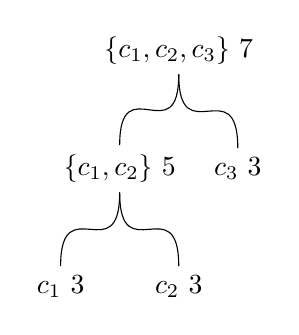
\begin{tikzpicture}[edge from parent path= 
  {(\tikzparentnode.south) .. controls +(0,-1) and +(0,1) 
                           .. (\tikzchildnode.north)}] 
  \node {$\{c_1,c_2,c_3\}$ 7}
    child { node {$\{c_1,c_2\}$ 5}  
	child{node {$c_1$ 3} }
	child{node {$c_2$ 3} } 
   }
    child { node {$c_3$ 3} };
\end{tikzpicture}
\end{minipage}%
 \begin{minipage}{.5\linewidth}
\centering
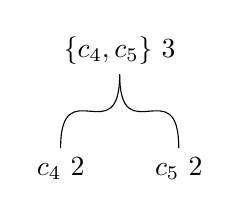
\begin{tikzpicture}[edge from parent path= 
  {(\tikzparentnode.south) .. controls +(0,-1) and +(0,1) 
                           .. (\tikzchildnode.north)}] 
  \node {$\{c_4,c_5\}$ 3}
    child { node {$c_4$ 2}  }
    child { node {$c_5$ 2} };
\end{tikzpicture}
\end{minipage}%
\caption{Bosque representando las restricciones del ejemplo \ref{ejeanidado}}
\end{figure}
Falta mencionar que en cada nodo aparece el conjunto de universidades junto con su cota superior. El nodo padre de cada árbol es el \textbf{grupo} de las universidades pertenecientes a ese árbol. \fin
\end{eje}

Existen varias definiciones nuevas que nos gustaría agregar al problema, para verlo en terminos más simples.
\begin{dfn}
Algunos terminos que utilizaremos son los siguientes:
\begin{enumerate}

\item Decimos que $M$ es la \textbf{función de emparejamiento} si dado una asignación $M$\footnote{El abuso de notación es para confundir al lector lo menos posible.} tenemos que para un aplicante $a$ arbitrario, $M(a)$ es la universidad a la que es asignado es $M$ y  conjunto de universidades $c$ arbitrario, $M(c)$ es el conjunto de aplicantes asignados a $b$ en $M$.
\item Decimos un conjunto de universidades $c$ está \textbf{lleno} si la cardinalidad de $M(c)$ es igual a $q(c)$. 
\item Decimos que un conjunto de universidades esta \textbf{subsuscrito} si no esta lleno. 
\item Una universidad esta \textbf{libre} si ningun conjunto que la contiene esta lleno, es lo mismo a que su grupo esta libre. Si no esta libre decimos que esta \textbf{restringida}. Las universidades libres pueden admitir a uno o más aplicantes sin violar ninguna restricción. 
\item Dada una universidad $c$ restringida dada un emparejamiento $M$, decimos que $Cs_M(c)$ es el \textbf{conjunto critico} de $c$ dado $M$ si es el conjunto de universidades lleno minimal que contiene a $c$. Esto quiere decir que dado el árbol de restricciones donde aparece $c$, $Cs_M(c)$ es el nodo padre de $c$ más abajo (no existen nodos llenos entre el y $c$) con la propiedad de que esta lleno. 
\end{enumerate}
\end{dfn}

%El siguiente ejemplo es para dejar todo un poco más claro. 

%\begin{eje}
%Me da flojera pero es agarrar el ejemplo de arriba y aplicar definiciones
%\end{eje}

Este problema difiere con el del capítulo 7 en el sentido de que si es facil de resolver. A continuación esta un algoritmo de cómo llegar a una asignación estable para el problema, mostraremos su convergencia y su veremos cuál es su complejidad. Al igual que en el capítulo 3 veremos que hay algoritmos optimos para los aplicantes y algortimos optimos para las unviersidades, se muestra primero el de los aplicantes. %no mames este parrafo. 

\section{Algoritmo orientado a los aplicantes}

\IncMargin{1em}
\begin{Algoritmo}[H]
%\SetKwData{Left}{left}\SetKwData{This}{this}\SetKwData{Up}{up}
%\SetKwFunction{Union}{Union}\SetKwFunction{FindCompress}{FindCompress}
\SetKwInOut{Input}{input}\SetKwInOut{Output}{output}

\Input{Lista de restricciones y preferencias de las universidades y los aplicantes }
\Output{Un emparejamiento.}
\BlankLine
\While{ Existe un aplicante $a$ que no esta emparejado y que no haya sido rechazado por todas las universidades.}{
		\emph{$c$ es la primera universidad de la lista de $a$ a la que no ha aplicado;} \\
		\If{$c$ esta libre}{\emph{asignamos $a$ a $c$;}}
		\Else{\emph{Sea $S$ el conjunto critico de $C$;} \\
		\If{Si $a$ es preferido en la lista del grupo de $c$ al pero aplicante $b$ que esta asignado en alguna universidad en $S$}{
			\emph{Sea $d$ la universidad a la que esta asignado $b$;} \\
			\emph{Eliminamos $(b,d)$ del emparejamiento;}\\
			\emph{Agregamos $(a,c)$ al emparejamiento;}
}
\Else{$a$ es rechazado por $c$;}			
}		
}
\caption{Algoritmo orientado a los aplicantes}
\end{Algoritmo}
\DecMargin{1em}

Los siguientes resultados hablan sobre la convergencia y complejidad del algoritmo.

\begin{lem}
\label{lemaAOA1}
Si alguna universidad $c$ en el algun punto del algoritmo orientado a los aplicantes queda restringida, entonces no vuelve a estar libre.
\end{lem}
\begin{proof}
En cualquier iteración del algoritmo si alguna universidad $c$ con un conjunto critico $S$, si el conjunto $S$ que subsuscrito seria porque alguna universidad en $S$ rechazo a algun aplicante actual $a$. Si esto sucede es porque algun conjunto $S'$
 que contiene a $S$ estaba lleno y rechazo a $a$ para aceptar a un mejor aplicante en su lista. De esta forma $c$ queda restrungida por $S'$.
\end{proof}

\begin{lem}
\label{lemaAOA2}
Si $M$ es un emparejamiento bajo el cual $c$ esta restringido y $M'$ es el emparejamiento obtenido en el siguiente paso del algoritmo orientado a los aplicantes. Entonces, el aplicante más abajo en la lista en  $Cs_{M'}(c)$ no puede ser menos preferido que el menos preferido en $Cs_M(c)$.
\end{lem}
\begin{proof}
Primero notamos que el si $S$ y $S'$ son dos conjuntos de universidades y $S$ es un subconjunto de $S'$ entonces el peor aplicante en $S$ esta a lo más igual de alto en la lista de preferencias que el peor aplicante en $S'$. \\
Supongamos que en el siguiente paso de algoritmo, el aplicante $b$ aplica a la universidad $d$ y es rechazado, como $M'$ queda identico a $M$ el lema queda como verdadero para este caso. \\
En el otro caso, supongamos que $d$ acepta a $b$ para ser parte de su universidad. Sea $S$ el conjunto critico de $c$ en el emparejamiento $M$, sea $S'$ el conjunto critico en $S'$, sea $T$ el conjunto critico de $d$ en $M'$. Consideramos cinco casos:
\begin{enumerate}
\item Supongamos $d$ estaba libre en $M$, esto implica directamente que $S=S'$ y el resultado sigue de esto.
\item Supongamos que la intersección entre $S$ y $T$ es igual al vacío, de aquí sale directo que en la iteración $S$ no cambia y por lo tanto $S=S'$ y el resultado sigue de esto.
\item Supongamos que $T$ es un subconjunto propio de $S$, entonces $c$ n o pertenece a $T$ (porque esto contradijería la hipotesis de que $S$ es el conjunto critico de $c$). De aquí sigue que $S=S'$ y como los cambios de $M$  a $M'$ solo suceden en $T$ los aplicantes emparejados en $S\setminus T$ son los mismos a los asignados en $S' \setminus T$ y en T por como funciona el algoritmo el peor alumno asignado en $M'$ debe de ser mejor al peor alumno asigando en $M$. De aquí se sigue que esto es cierto para $S$ y $S'$.
\item Supongamos que $T$ es igual a $S$. Aquí tenemos que la cantidad de alumnos asignados bajo $M$ en $S$ son iguales a la cantidad de alumnos asiganos bajo $M'$ a $S$ y simultaneamente son iguales a la cota superior de $S$. En este caso existe la posibilidad de que $S'$ sea un subconjunto de $S$ pero por la observación realizada al principio de la demostración concluimos que para este caso el lema es verdadero.
\item Por ultimo, supongamos que $S$ es un subconjunto propio de $T$. Si el aplicante rechazado no se encontraba asignado en $S$ entonces el resultado se sigue directo de que los asignados en $S$ bajo $M$ y en $S'$ bajo $M'$ no cambian. En otro caso, debe de suceder que la cantidad de alumnos asignados en $S$ bajo $M'$ son estrictamente menores a la cantidad de alumnos asignados a $S$ bajo $M$ y que esto además sucede para toda $S^*$ con la propiedad de que $S$ es un subconjunto de $S^*$, $S^*$ es un subconjunto de $T$ y $d$ no pertenece a $S^*$. Además sabemos que la cantidad de alumnos asignados bajo $M$ son iguales a la cantidad de alumnos asiganos bajo $M'$ a toda $S^*$ que cumple que $S$ es un subconjunto de $S^*$, $S^*$ es un subconjunto de $T$ y $d$ pertenece a $S^*$, pero la cantidad de alumnos asignados es estrictamente menor a su cota superior.  Esto implica que el nuevo conjunto critico de $c$ ($S'$) es igual a $T$, como $S'$ es el conjunto critico de $d$ y en la iteración del algoritmo rechazo a su peor aplicante, se sigue que el lema es correcto para este caso. 
\end{enumerate}
Por lo tanto, Si $M$ es un emparejamiento bajo el cual $c$ esta restringido y $M'$ es el emparejamiento obtenido en el siguiente paso del algoritmo orientado a los aplicantes. Entonces, el aplicante más abajo en la lista en  $Cs_{M'}(c)$ no puede ser menos preferido que el menos preferido en $Cs_M(c)$.
\end{proof}

El siguiente teorema habla de la convergencia de este algoritmo y muestra un resultado en terminos de optimalidad.

\begin{teo}
Dado un problema de admisión a universidades con cotas comunes anidadas, el emparejamiento $M$ encontrado por el algoritmo orientado a los aplicantes es estable y además cumple que cada aplicante se encuentra en la mejor asignación posible que en cualquier otra asignación estable.
\end{teo}

\begin{proof}
Supongamos que $M$ no es estable y por lo tanto existe un aplicante $a$ y una universidad $c$ que se prefieren a su asignación actual. Como $a$ prefiere a $c$, podemos ver que $c$ rechazo a $a$ en algun paso del algoritmo. En esa iteración dek algoritmo $c$ estaba restringida y prefirio a algun aplicante $b$ ($b$ aquí siendo el menos preferido entre los asignados) sobre $a$ (de acuerdo a lista de su grupo). Por los lemas \ref{lemaAOA1} y \ref{lemaAOA1} $c$ se mantiene restringida en las iteraciones posteriores y el peor aplicante de su conjunto critico no puede ser menos preferido que $b$. Por lo tanto, llegamos a una contradicción y concluimos que $M$ es estable. \\
Ahora, supongamos que el algoritmo no es optimo para los aplicantes eso es existen un aplicante $a$ y una universidad $c$ emparejados en $M$, además existe otra asignación estable $M'$ en donde $a$ esta asignado a $c'$ y $a$ prefiere a $c'$ sobre $c$ (adicional a esto supongamos que en algoritmo es la primera asignación estable que es rechazada). Como $a$ prefiere a $c'$ podemos concluir que $c'$ rechazo a $a$ en algun punto del algoritmo. \\
Sea $X$ el emparejamiento obtenido antes de que un aplicante $a^*$ aplicara a alguna universidad $c^*$ resultando en que $c'$ rechazara a $a$. Sea $S=Cs_X(c^*)$ el conjunto critico de $c^*$ en $X$ y sea $X^*=X \cup \{(a^*,c^*)\}$. Mostraremos que existe yn aplicante $d$ y una unversidad $d$ tales que:
\begin{enumerate}
\item $d$ esta asignado a $b$ en $X^*$.
\item $b$ no esta asignado a $d$ en $M'$.
\item $d$ esta libre en $M'$ o $S$ es un subconujunto de $Cs_{M'}(d)$.
\end{enumerate}
Primero, notamos que la cantidad de alumnos asignados a $S$ en $M'$ es menor o igual que la cota de $S$ que esta a su vez igual a la cantidad de alumnos asignados a $S$ en $X$. Además podemos ver que la cantidad de alumnos asignados a $S$ en $X^*$ excede a la cota superior de $S$ por 1, como la cota se excede a partir de agregar un nuevo par podemos ver que para cualquier subconjunto propio $S_i$ de $S$ se cumple que la cantidad de personadas asignadas a $S_i$ en $X^*$ es menor o igual a la cota de $S_i$ (porque $S=Cs_X(c^*)$), por lo tanto $S$ es es el conjunto minimal que no cumple la cota. Esto implica que alguno de sus hijos (en el sentido de las restricciones) $S_2$ satisface que la cantidad de personas emparejadas en $M'$ es menor estricto a la cantidad de personas emparejadas en $X^*$ que es menor igual a su cota. Por la misma razon, podemos construir una sucesión en donde $S=S_1$, $S_{i+1}$ es un subconjunto propio de $S_i$, $S_{k}$ es igual a $\{d\}$ y cada $S_i$ satisface la propiedad anterior. Finalmente sea $b$ el aplicante que se encuentra asignado en $X^*$ a $d$ pero en $M'$. \\
Ahora, notamos que $b$ esta en mejor posición que $a$, de otra forma en la siguiente iteración del algoritmo hubieran rechazado a $b$ y no a $a$. Entonces, como $b$ no esta asignado en $M'$ o prefiere a $d$ que a su respectiva universidad en $M'$, como $S$ es un subconjunto de  $Cs_{M'}(d)$ se sigue que la pareja $(b,d)$ ocasiona que $M'$ no sea estable. Por lo tanto llegamos a una contradicción y concluimos que el algoritmo es optimo para los aplicantes. 
\end{proof}

Además a esto podemos ver que el algoritmo siempre es consistente sin importar en que orden se itere. 

\begin{cor}
Cualquier ejecución del algoritmo orientado a los aplicantes llega a la misma asignación estable. 
\end{cor}
\begin{proof}
Como el algoritmo es optimo sin importar el orden sobre el que se itera, podemos concluir que siempre se llega a la misma asignación estable.
\end{proof}

A partir de esto podemos estudiar cuál es la diferencia principal entre pedir que las cotas comunes sean anidadas y no tener ninguna restricción sobre estas. El siguiente resultado muestra como el comportamiento de este problema es mucho más amigable en terminos algoritmicos. 

\begin{teo}
La complejidad del algoritmo orientado a los aplicantes es del orden de $kL+pn$ donde $L$ es la cantidad de parejas aceptables, $k$ es la longitud máxima de algun árbol en el bosque de restricciones, $n$ es el número de aplicantes y $p$ e el número de conjuntos acotados. 
\end{teo}
\begin{proof}
El primer termino viene de que el primer %``loop´´ del algoritmo es realiza en un orden $L$ veces y con la excepción de actualizar el peor aplicante cada paso en el ``loop´´ es realizado en un orden de $k$ veces. 
% No tengo paciencia
\end{proof}


\section{Algoritmo orientado a las universidades}

Igual que en el caso del matrimonio estable la idea de optimalidad para los aplicantes se puede reorientar a optimalidad para las universidades, usualmente las que escojen con que alumnos quedarse son las universidades y resulta más intuitiva este tipo de optimalidad. En lo que sigue del capitulo se muestra un algoritmo y se muestran algunos resultados sobre el mismo. Para empezar es necesario explicar las siguientes definiciones:
\begin{enumerate}
\item Decimos que un aplicante es \textbf{no tratado} para un conjunto $S$ si ninguna universidad en $S$ le ha ofrecido un puesto.
\item Sea $a$ algun aplicante que es no tratado por alguna universidad libre $c$ en $G$. Decimos que la pareja $(c,a)$ constituye una \textbf{oferta lider}.
\end{enumerate}

A continuación mostramos el algoritmo orientado a las universidades, la diferencia importante entre este algoritmo y el otro es que aquí las universidades le ofrecen los puestos a los alumnos y no al revez.

\IncMargin{1em}
\begin{Algoritmo}[H]
%\SetKwData{Left}{left}\SetKwData{This}{this}\SetKwData{Up}{up}
%\SetKwFunction{Union}{Union}\SetKwFunction{FindCompress}{FindCompress}
\SetKwInOut{Input}{input}\SetKwInOut{Output}{output}

\Input{Lista de restricciones y preferencias de las universidades y los aplicantes }
\Output{Un emparejamiento.}
\BlankLine
\While{ Existe un grupo de universidades $G$ que este subsuscrito y existe una universidad libre con un aplicante no tratado.}{
		\emph{Sea $(c,a)$ la oferta lider en ese punto;}
		\emph{Marcamos a $a$ como tratado por $c$;}
\If{$a$ no esta asignado}{Agregamos $(a,c)$ a la asignación;}
\Else{

\If{$a$ prefiere a $c$ que a su univerdiad actual $d$}{
	\emph{Quitamos a $(a,d)$ del emparejamiento;}
	\emph{Agregamos $(a,c)$ a la asignación;}
}
\Else{$a$ rechaza a $c$;}
}
}
\caption{Algoritmo orientado a las universidades}
\end{Algoritmo}
\DecMargin{1em}

El siguiente lema y teorema nos ayudan a entender qué tan bueno es este algoritmo y cuál es la diferencia central con el algoritmo orientado a los aplicantes. 


\begin{lem}
Si en algun punto del algoritmo, una universidad $d$ en un grupo $G$ le ofrece un puesto a un aplicante $b$ entonces si se cumple alguna de las siguientes dos cosas:
\begin{enumerate}
\item Si a algun otro aplicante $a$ (superior a $b$ en la lista de $G$) no se le ofrece un puesto en alguna universidad $c$ en $G$, donde $a$ es no es marcado como tratado por $c$.
\item Si a $b$ no le ofrecen un puesto en $c$ (superior a $d$ en la lista de $b$), donde $b$ no es marcado como tratado por $c$.
\end{enumerate}
Entonces, $c$ esta restringido y su conjunto critico no se encuentra en el camino entre $d$ y la parte de arriba del árbol.
\end{lem}
\begin{proof}
Por la definición de la oferta lider podemos directamente concluir que $c$ esta restringido. Como $d$ esta libre (por hipotesis) sabemos que no es parte de ningun conjunto restringido y por lo tanto tampoco de algun conjunto critico.
\end{proof}
\begin{teo}
El emperajamiento $M$ obtenido por el algoritmo orientado a las universidades es estable. Si algun aplicante $a$ queda asignado a alguna universidad $c$ en $M$, entonces no existe otra asignación estable en la que $a$ no quede emparejado o en la que quede asignado a una peor universidad en su lista. Si alguna universidad $c$ tiene asignados a $a_1,a_2,\dots,a_k$ en $M$, entonces no existe ningun aplicante $a$ mejor  que ellos en ningun otro emparejamiento estable.
\end{teo}
\begin{proof}
Supongamos que $M$ es no estable y que es bloqueado por un aplicante $a$ y una universidad $c$, esto es que ambos se prefieren a sus respectivas asingaciones. Sabgemos que $c$ no le ofrecio un lugar a $a$ durante el algoritmo porque los aplicantes solo pueden mejorar mientras progesa el algortimo (no haria sentido que empeoren). De aquí sigue que $c$ debe tener un conjunto critico $S$ al finalizar el algoritmo.\\
Como $(a,c)$ bloquean la estabilidad entonces deben de existir una universidad $d$ en $S$ y un aplicante $b$ que es asignado a $d$ en $M$ tal que $a$ es preferido a $b$ y $a$ prefiere a $c$ que a su asinación actual. Aquí la contradicción es clara porque $c$ debio de haber ofrecido un puesto primero a $a$ que a $b$ y como $a$ prefiere a $c$ entonces podemos concluir que $M$ es estable. \\
Supongamos que existe un emparejamiento estable $M'$ en donde existe un aplicante $a$ que no esta asignado o donde esta asignado a una peor universidad que en $M$ (supongamos que en $M$ esta asignado a $c$). Supongamos que cuando a $c$ le ofrecio un puesto a $a$ esta fue la primera que un aplicante recibio una oferta que era mejor a su estatus en otra asignación estable. Llamaremos a esta oferta \textbf{superior}. Para evitar que $(a,c)$ bloquee la estabilidad de $M'$ es necesario suponer que el conjunto critico de $c$ en $M'$ esta lleno con aplicantes superiores a $a$. \\
Sea $M^*$ el emparejamiento obtenido por el algoritmo antes de ofrecerle un puesta a $a$ en $c$. Como $c$ estaba libre en ese momento sabemos que la cantidad de alumnos asignados a $S$ en $M^*$ en ese momento era menor estrico que la cantidad de personas asignadas a $S$ en $M'$ que esta a su vez es igual a la cota superior de $S$. Esto implica que algun hijo $S_2$ de $S$ cumple que la cantidad de personas asignadas a $S_2$ en $M^*$ es menor a la cantidad de personas asignadas en $M'$ que esta a su vez es menor o igual a la cota de $S_2$. Con el mismo razonamiento podemos construir una sucesión en donde $S=S_1$, $S_{i+1}$ es un subconjunto propio de $S_i$, $S_{k}$ es igual a $\{d\}$ y cada $S_i$ satisface la propiedad anterior. FInalmente sea $b$ algun aplicante asignado a $d$ en $M'$ pero no en $M^*$. Se sigue de la construcción que $d$ es libre en $M^*$ y que $b$ esta mejor calificada que $a$. Por lo tanto, $b$ debe de estar emparejada en $M^*$ con una universidad $e$ a la que prefiere sobre $d$. Por lo tanto, $d$ recibio una oferta de $e$ antes que $a$ de $c$, lo que contradice el supuesto de que fue el primer aplicante que recibio una oferta que era mejor a su estatus en otra asignación estable. Podemos concluor que $a$ no esta asignado a una peor universidad que $c$ en ningun otro emparejamiento estable y que no existe algun emparejamiento estable en el que $a$ no este asignado. \\
Finalmente, supongamos ahora que a esta asignado a $c$ en $M$ y que $b$ no esta asignado a $c$ en $M$ pero si en otro emparejamiento estable $M'$ y que $b$ esta más arriba en la lista de preferencias que $a$. Entonces por el argumento de arriba $b$ debe de preferir a $c$ sobre su asignación en $M$ o no esta asignada, de aquí sigue que $(b,c)$ bloquea la estabilidad de $M$ y por lo tanto llegamos a una contradicción. 
\end{proof}

Hablar de complejidad

Para dejar más clara la diferencia entre los dos algoritmos mostramos el siguiente ejemplo.

\begin{eje}
Retomamos las restricciones mostradas en el ejemplo \ref{ejeanidado} y agregamos las siguientes listas de preferencias:


 \begin{minipage}{.25\linewidth}
$$P(a_1)=c_1 c_2$$ \\
$$P(a_5)=c_5 c_3$$ \\
$$P(a_9)= c_4 c_1$$
\end{minipage}%
\begin{minipage}{.25\linewidth}
$$P(a_2)= c_1 c_4$$ \\
$$P(a_6)=c_3 c_4$$  \\
$$P(a_{10})=c_2 c_4 c_5$$
\end{minipage}
\begin{minipage}{.25\linewidth}
$$P(a_3)= c_2 c_1$$ \\
$$P(a_7)=c_1 c_4 c_5$$ 
\end{minipage}
\begin{minipage}{.25\linewidth}
$$P(a_4)=c_2 c_4$$ \\
$$P(a_8)=c_2 c_1$$ 
\end{minipage}

El algoritmo orientado a los aplicantes sigue de acuerdo a los siguientes pasos \footnote{se modifico un poco el orden con respecto al codigo para efectos de la explicación}.
\begin{figure}[H]
\begin{minipage}{.5\linewidth}
\begin{figure}[H]\centering

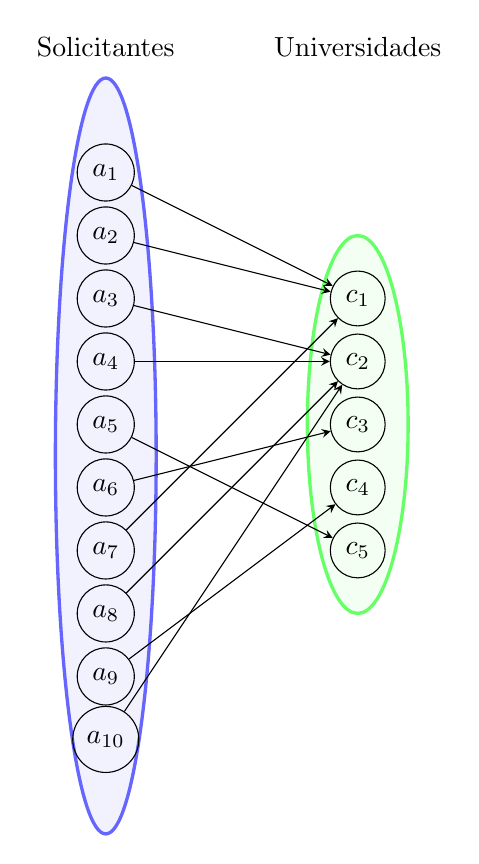
\begin{tikzpicture}[ scale=0.8]
\tikzset{vertex/.style = {shape=circle,draw,minimum size=1.5em}}
\tikzset{edge/.style = {->,> = latex}}


\filldraw[color=blue!60, fill=blue!5, very thick](0,-.5) ellipse (.8 and 6);
\filldraw[color=green!60, fill=green!5, very thick](4,0) ellipse (.8 and 3);


% vertices
% 

\node[vertex] (a) at (4,2) {$c_1$};
\node[vertex] (b) at (4,1) {$c_2$};
\node[vertex] (c) at (4,0) {$c_3$};
\node[vertex] (d) at (4,-1) {$c_4$};
\node[vertex] (e) at (4,-2) {$c_5$};


\node[vertex] (g) at (0,4) {$a_1$};
\node[vertex] (h) at (0,3) {$a_2$};
\node[vertex] (i) at (0,2) {$a_3$};
\node[vertex] (j) at (0,1) {$a_4$};
\node[vertex] (k) at (0,0) {$a_5$};
\node[vertex] (l) at (0,-1) {$a_6$};
\node[vertex] (m) at (0,-2) {$a_7$};
\node[vertex] (n) at (0,-3) {$a_8$};
\node[vertex] (o) at (0,-4) {$a_9$};
\node[vertex] (p) at (0,-5) {$a_{10}$};


\node (w) at (0,6) {Solicitantes};
\node (x) at (4,6) {Universidades};

\path[-stealth] (g) edge (a);
\path[-stealth] (h) edge (a);
\path[-stealth] (i) edge (b);
\path[-stealth] (j) edge (b);
\path[-stealth] (k) edge (e);
\path[-stealth] (l) edge (c);
\path[-stealth] (m) edge (a);
\path[-stealth] (n) edge (b);
\path[-stealth] (o) edge (d);
\path[-stealth] (p) edge (b);

%\path[-stealth] (b) edge (g);

%\draw (4,4) node[cross=8pt,red] {};


%\draw (0.2,8)--(3.8,8);



\end{tikzpicture}
%\caption{los 10 aplicantes aplican a su mejor universidad, $a_7$ y $a_10$ son rechazados porque $\{c_1,c_2\}$ esta lleno en el primer caso y en el segundo porque $c_2$ queda restringida.}
\end{figure}
\end{minipage}
\begin{minipage}{.5\linewidth}
\begin{figure}[H]\centering

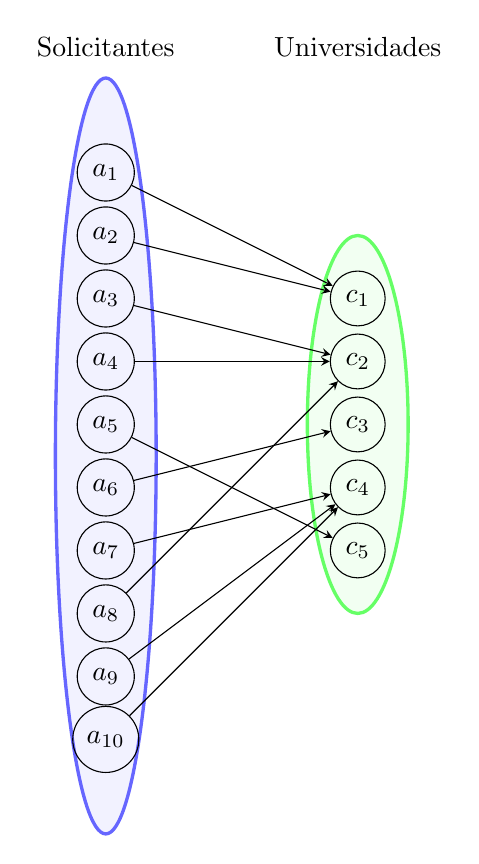
\begin{tikzpicture}[ scale=0.8]
\tikzset{vertex/.style = {shape=circle,draw,minimum size=1.5em}}
\tikzset{edge/.style = {->,> = latex}}


\filldraw[color=blue!60, fill=blue!5, very thick](0,-.5) ellipse (.8 and 6);
\filldraw[color=green!60, fill=green!5, very thick](4,0) ellipse (.8 and 3);


% vertices
% 
\node[vertex] (a) at (4,2) {$c_1$};
\node[vertex] (b) at (4,1) {$c_2$};
\node[vertex] (c) at (4,0) {$c_3$};
\node[vertex] (d) at (4,-1) {$c_4$};
\node[vertex] (e) at (4,-2) {$c_5$};


\node[vertex] (g) at (0,4) {$a_1$};
\node[vertex] (h) at (0,3) {$a_2$};
\node[vertex] (i) at (0,2) {$a_3$};
\node[vertex] (j) at (0,1) {$a_4$};
\node[vertex] (k) at (0,0) {$a_5$};
\node[vertex] (l) at (0,-1) {$a_6$};
\node[vertex] (m) at (0,-2) {$a_7$};
\node[vertex] (n) at (0,-3) {$a_8$};
\node[vertex] (o) at (0,-4) {$a_9$};
\node[vertex] (p) at (0,-5) {$a_{10}$};


\node (w) at (0,6) {Solicitantes};
\node (x) at (4,6) {Universidades};

\path[-stealth] (g) edge (a);
\path[-stealth] (h) edge (a);
\path[-stealth] (i) edge (b);
\path[-stealth] (j) edge (b);
\path[-stealth] (k) edge (e);
\path[-stealth] (l) edge (c);
\path[-stealth] (m) edge (d);
\path[-stealth] (n) edge (b);
\path[-stealth] (o) edge (d);
\path[-stealth] (p) edge (d);
%\path[-stealth] (b) edge (g);

%\draw (4,4) node[cross=8pt,red] {};


%\draw (0.2,8)--(3.8,8);



\end{tikzpicture}
%\caption{ $a_7$ aplica a $c_4$ y $a_{10}$  aplica a $c_4$, $a_10$ es rechazado porque $c_4$ queda restringida.}
\end{figure}
\end{minipage}

%\caption{Aginaciones estables.}
\end{figure}

Los 10 aplicantes aplican a su mejor universidad, $a_7$ y $a_10$ son rechazados porque $\{c_1,c_2\}$ esta lleno en el primer caso y en el segundo porque $c_2$ queda restringida. $a_7$ aplica a $c_4$ y $a_{10}$  aplica a $c_4$, $a_10$ es rechazado porque $c_4$ queda restringida.


\begin{figure}[H]
\begin{minipage}{.5\linewidth}
\begin{figure}[H]\centering

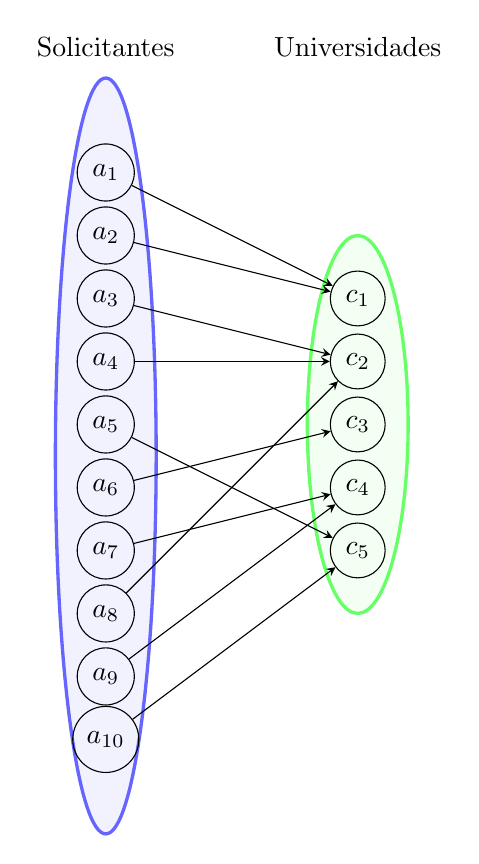
\begin{tikzpicture}[ scale=0.8]
\tikzset{vertex/.style = {shape=circle,draw,minimum size=1.5em}}
\tikzset{edge/.style = {->,> = latex}}


\filldraw[color=blue!60, fill=blue!5, very thick](0,-.5) ellipse (.8 and 6);
\filldraw[color=green!60, fill=green!5, very thick](4,0) ellipse (.8 and 3);


% vertices
% 

\node[vertex] (a) at (4,2) {$c_1$};
\node[vertex] (b) at (4,1) {$c_2$};
\node[vertex] (c) at (4,0) {$c_3$};
\node[vertex] (d) at (4,-1) {$c_4$};
\node[vertex] (e) at (4,-2) {$c_5$};


\node[vertex] (g) at (0,4) {$a_1$};
\node[vertex] (h) at (0,3) {$a_2$};
\node[vertex] (i) at (0,2) {$a_3$};
\node[vertex] (j) at (0,1) {$a_4$};
\node[vertex] (k) at (0,0) {$a_5$};
\node[vertex] (l) at (0,-1) {$a_6$};
\node[vertex] (m) at (0,-2) {$a_7$};
\node[vertex] (n) at (0,-3) {$a_8$};
\node[vertex] (o) at (0,-4) {$a_9$};
\node[vertex] (p) at (0,-5) {$a_{10}$};


\node (w) at (0,6) {Solicitantes};
\node (x) at (4,6) {Universidades};

\path[-stealth] (g) edge (a);
\path[-stealth] (h) edge (a);
\path[-stealth] (i) edge (b);
\path[-stealth] (j) edge (b);
\path[-stealth] (k) edge (e);
\path[-stealth] (l) edge (c);
\path[-stealth] (m) edge (d);
\path[-stealth] (n) edge (b);
\path[-stealth] (o) edge (d);
\path[-stealth] (p) edge (e);

%\path[-stealth] (b) edge (g);

%\draw (4,4) node[cross=8pt,red] {};


%\draw (0.2,8)--(3.8,8);



\end{tikzpicture}
%\caption{los 10 aplicantes aplican a su mejor universidad, $a_7$ y $a_10$ son rechazados porque $\{c_1,c_2\}$ esta lleno en el primer caso y en el segundo porque $c_2$ queda restringida.}
\end{figure}
\end{minipage}
\begin{minipage}{.5\linewidth}
\begin{figure}[H]\centering

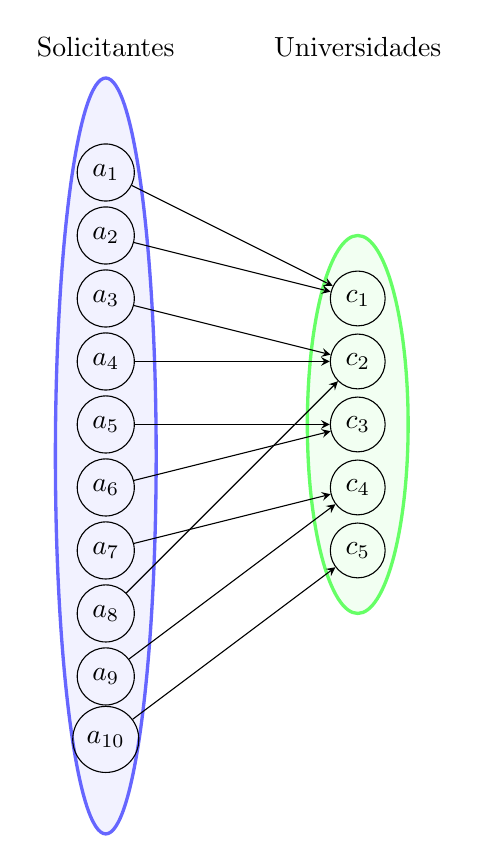
\begin{tikzpicture}[ scale=0.8]
\tikzset{vertex/.style = {shape=circle,draw,minimum size=1.5em}}
\tikzset{edge/.style = {->,> = latex}}


\filldraw[color=blue!60, fill=blue!5, very thick](0,-.5) ellipse (.8 and 6);
\filldraw[color=green!60, fill=green!5, very thick](4,0) ellipse (.8 and 3);


% vertices
% 
\node[vertex] (a) at (4,2) {$c_1$};
\node[vertex] (b) at (4,1) {$c_2$};
\node[vertex] (c) at (4,0) {$c_3$};
\node[vertex] (d) at (4,-1) {$c_4$};
\node[vertex] (e) at (4,-2) {$c_5$};


\node[vertex] (g) at (0,4) {$a_1$};
\node[vertex] (h) at (0,3) {$a_2$};
\node[vertex] (i) at (0,2) {$a_3$};
\node[vertex] (j) at (0,1) {$a_4$};
\node[vertex] (k) at (0,0) {$a_5$};
\node[vertex] (l) at (0,-1) {$a_6$};
\node[vertex] (m) at (0,-2) {$a_7$};
\node[vertex] (n) at (0,-3) {$a_8$};
\node[vertex] (o) at (0,-4) {$a_9$};
\node[vertex] (p) at (0,-5) {$a_{10}$};


\node (w) at (0,6) {Solicitantes};
\node (x) at (4,6) {Universidades};

\path[-stealth] (g) edge (a);
\path[-stealth] (h) edge (a);
\path[-stealth] (i) edge (b);
\path[-stealth] (j) edge (b);
\path[-stealth] (k) edge (c);
\path[-stealth] (l) edge (c);
\path[-stealth] (m) edge (d);
\path[-stealth] (n) edge (b);
\path[-stealth] (o) edge (d);
\path[-stealth] (p) edge (e);
%\path[-stealth] (b) edge (g);

%\draw (4,4) node[cross=8pt,red] {};


%\draw (0.2,8)--(3.8,8);



\end{tikzpicture}
%\caption{ $a_7$ aplica a $c_4$ y $a_{10}$  aplica a $c_4$, $a_10$ es rechazado porque $c_4$ queda restringida.}
\end{figure}
\end{minipage}

%\caption{Aginaciones estables.}
\end{figure}

$a_10$ aplica a $c_5$, $c_5$ acepta a $a_10$ y rechaza a $a_5$ porque $\{c_4,c_5\}$ queda lleno. $a_5$ aplica a $c_3$ y es aceptada. El algoritmo finaliza.

El algoritmo orientado a las universidades sigue de acuerdo a los siguientes pasos \footnote{se modifico un poco el orden con respecto al codigo para efectos de la explicación}.

\begin{figure}[H]
\begin{minipage}{.5\linewidth}
\begin{figure}[H]\centering

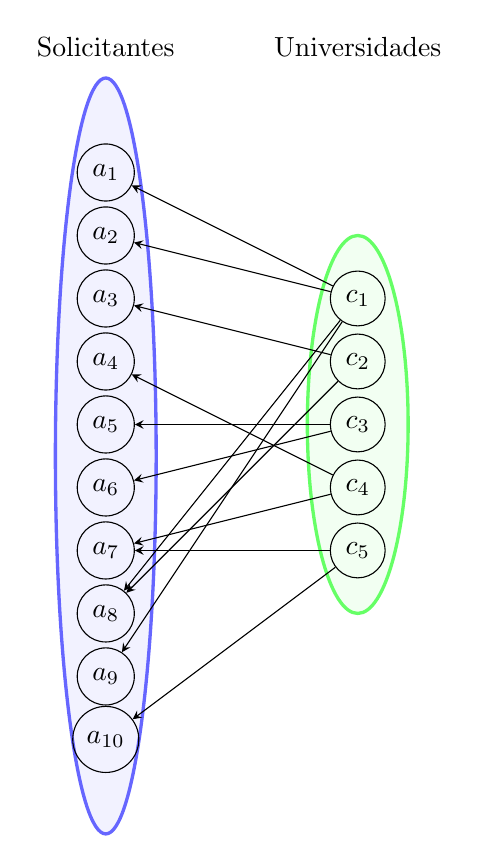
\begin{tikzpicture}[ scale=0.8]
\tikzset{vertex/.style = {shape=circle,draw,minimum size=1.5em}}
\tikzset{edge/.style = {->,> = latex}}


\filldraw[color=blue!60, fill=blue!5, very thick](0,-.5) ellipse (.8 and 6);
\filldraw[color=green!60, fill=green!5, very thick](4,0) ellipse (.8 and 3);


% vertices
% 

\node[vertex] (a) at (4,2) {$c_1$};
\node[vertex] (b) at (4,1) {$c_2$};
\node[vertex] (c) at (4,0) {$c_3$};
\node[vertex] (d) at (4,-1) {$c_4$};
\node[vertex] (e) at (4,-2) {$c_5$};


\node[vertex] (g) at (0,4) {$a_1$};
\node[vertex] (h) at (0,3) {$a_2$};
\node[vertex] (i) at (0,2) {$a_3$};
\node[vertex] (j) at (0,1) {$a_4$};
\node[vertex] (k) at (0,0) {$a_5$};
\node[vertex] (l) at (0,-1) {$a_6$};
\node[vertex] (m) at (0,-2) {$a_7$};
\node[vertex] (n) at (0,-3) {$a_8$};
\node[vertex] (o) at (0,-4) {$a_9$};
\node[vertex] (p) at (0,-5) {$a_{10}$};


\node (w) at (0,6) {Solicitantes};
\node (x) at (4,6) {Universidades};

\path[-stealth] (b) edge (n);
\path[-stealth] (a) edge (n);
\path[-stealth] (a) edge (o);
\path[-stealth] (a) edge (g);
\path[-stealth] (a) edge (h);
\path[-stealth] (b) edge (i);
\path[-stealth] (c) edge (k);
\path[-stealth] (c) edge (l);
\path[-stealth] (d) edge (j);
\path[-stealth] (d) edge (m);
\path[-stealth] (e) edge (m);
\path[-stealth] (e) edge (p);


%\path[-stealth] (b) edge (g);

%\draw (4,4) node[cross=8pt,red] {};


%\draw (0.2,8)--(3.8,8);



\end{tikzpicture}
%\caption{los 10 aplicantes aplican a su mejor universidad, $a_7$ y $a_10$ son rechazados porque $\{c_1,c_2\}$ esta lleno en el primer caso y en el segundo porque $c_2$ queda restringida.}
\end{figure}
\end{minipage}
\begin{minipage}{.5\linewidth}
\begin{figure}[H]\centering

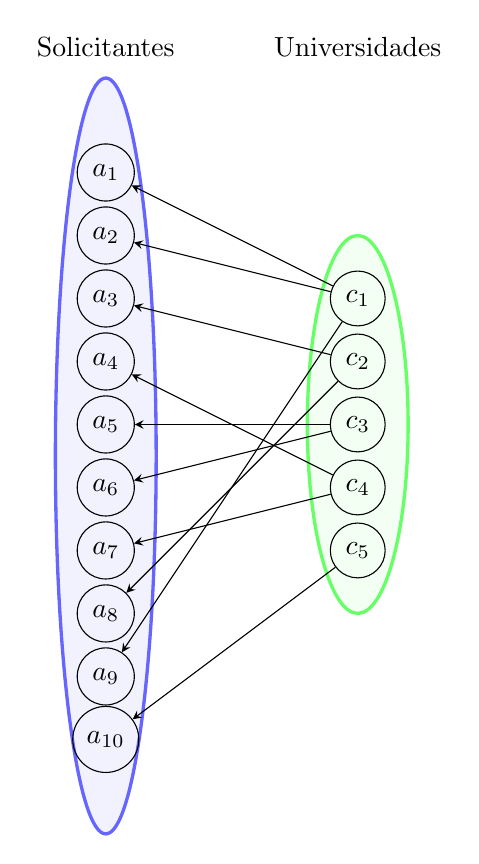
\begin{tikzpicture}[ scale=0.8]
\tikzset{vertex/.style = {shape=circle,draw,minimum size=1.5em}}
\tikzset{edge/.style = {->,> = latex}}


\filldraw[color=blue!60, fill=blue!5, very thick](0,-.5) ellipse (.8 and 6);
\filldraw[color=green!60, fill=green!5, very thick](4,0) ellipse (.8 and 3);


% vertices
% 
\node[vertex] (a) at (4,2) {$c_1$};
\node[vertex] (b) at (4,1) {$c_2$};
\node[vertex] (c) at (4,0) {$c_3$};
\node[vertex] (d) at (4,-1) {$c_4$};
\node[vertex] (e) at (4,-2) {$c_5$};


\node[vertex] (g) at (0,4) {$a_1$};
\node[vertex] (h) at (0,3) {$a_2$};
\node[vertex] (i) at (0,2) {$a_3$};
\node[vertex] (j) at (0,1) {$a_4$};
\node[vertex] (k) at (0,0) {$a_5$};
\node[vertex] (l) at (0,-1) {$a_6$};
\node[vertex] (m) at (0,-2) {$a_7$};
\node[vertex] (n) at (0,-3) {$a_8$};
\node[vertex] (o) at (0,-4) {$a_9$};
\node[vertex] (p) at (0,-5) {$a_{10}$};


\node (w) at (0,6) {Solicitantes};
\node (x) at (4,6) {Universidades};


\path[-stealth] (b) edge (n);
%\path[-stealth] (a) edge (n);
\path[-stealth] (a) edge (o);
\path[-stealth] (a) edge (g);
\path[-stealth] (a) edge (h);
\path[-stealth] (b) edge (i);
\path[-stealth] (c) edge (k);
\path[-stealth] (c) edge (l);
\path[-stealth] (d) edge (j);
\path[-stealth] (d) edge (m);
%\path[-stealth] (e) edge (m);
\path[-stealth] (e) edge (p);
%\draw (4,4) node[cross=8pt,red] {};


%\draw (0.2,8)--(3.8,8);



\end{tikzpicture}
%\caption{ $a_7$ aplica a $c_4$ y $a_{10}$  aplica a $c_4$, $a_10$ es rechazado porque $c_4$ queda restringida.}
\end{figure}
\end{minipage}

%\caption{Aginaciones estables.}
\end{figure}

Las 5 universidades invitan a los alumnos, $a_8$ rechaza a $c_1$ porque prefiere estar en $c_2$ y $a_7$ rechaza a $c_5$ porque prefiere a $c_4$. El algoritmo finaliza despues de esos pasos.

\fin

\end{eje}

Una nota importante es que en los emparejamientos $c_1$ y $c_2$ tienen un número distino de alumnos y por lo tanto en este caso no se cumple de la misma manera el teorema de los hospitales rurales. 

En lo que sigue de la tesis se introduce una estructura algebraica llamada matroide y se muestran resultados estructurales de este problema.


